\documentclass[acmsmall,10pt,anonymous]{acmart}
\settopmatter{printfolios=true,printccs=false,printacmref=false}
%% For double-blind review submission, w/ CCS and ACM Reference
%\documentclass[acmsmall,review,anonymous]{acmart}\settopmatter{printfolios=true}
%% For single-blind review submission, w/o CCS and ACM Reference (max submission space)
%\documentclass[acmsmall,review]{acmart}\settopmatter{printfolios=true,printccs=false,printacmref=false}
%% For single-blind review submission, w/ CCS and ACM Reference
%\documentclass[acmsmall,review]{acmart}\settopmatter{printfolios=true}
%% For final camera-ready submission, w/ required CCS and ACM Reference
%\documentclass[acmsmall]{acmart}\settopmatter{}

% Journal information
%% Supplied to authors by publisher for camera-ready submission;
%% use defaults for review submission.
\acmJournal{PACMPL}
\acmVolume{1}
\acmNumber{CONF} % CONF = POPL or ICFP or OOPSLA
\acmYear{2022}
\acmMonth{1}
\acmDOI{} % \acmDOI{10.1145/nnnnnnn.nnnnnnn}
% \startPage{1}

%% Copyright information
%% Supplied to authors (based on authors' rights management selection;
%% see authors.acm.org) by publisher for camera-ready submission;
%% use 'none' for review submission.
\setcopyright{none}
%\setcopyright{acmcopyright}
%\setcopyright{acmlicensed}
%\setcopyright{rightsretained}
%\copyrightyear{2018}           %% If different from \acmYear

\usepackage{trimclip}
\usepackage{graphicx}
\usepackage{float}
\usepackage{tikz}
\usepackage{tikz-cd}
\usetikzlibrary{
  positioning,
  shapes.geometric,
  arrows,
  arrows.meta,
  trees
}
\usepackage{mathpartir}
\usepackage{xcolor}
\usepackage{listings}
\usepackage[scaled=1.0]{beramono}
\usepackage{bm}
\usepackage[utf8x]{inputenc}
\usepackage[page,header]{appendix}
\usepackage{titletoc}
\usepackage{cleveref}
\usepackage{soul}

\tikzstyle{startstop} = [rectangle, minimum width=0.6cm, minimum height=0.8cm, text centered, draw=black]
\tikzstyle{process}   = [rectangle, minimum width=0.6cm, minimum height=0.8cm, text centered, text width=2.2cm, draw=black]
\tikzstyle{arrow}     = [thick,->,>=stealth]

\definecolor{codegreen}{rgb}{0,0.6,0}
\definecolor{eminence}{RGB}{108,48,130}

\lstdefinelanguage{tll}{
  emph={program, logical, theorem, def, inductive, where},
  morekeywords={let, let*, in, match, as, with, if, then, else, fork, fun, ln, fn},
  extendedchars=true, 
  alsoletter=*,
  morecomment=[l]{--},
  emphstyle=\color{blue},
  keywordstyle=\color{eminence},
  commentstyle=\color{codegreen},
  basicstyle=\footnotesize\ttfamily,
}

\lstnewenvironment{tllisting}{
\lstset{
  language=tll,
  basicstyle=\scriptsize\ttfamily,
  extendedchars=true,
  mathescape=true,
}}{}

\newcommand{\TODO}{\textbf{\textcolor{red}{TODO}}}

\newcommand{\mcA}{\mathcal{A}}
\newcommand{\mcF}{\mathcal{F}}
\newcommand{\mcP}{\mathcal{P}}
\newcommand{\mcE}{\mathcal{E}}
\newcommand{\mcM}{\mathcal{M}}
\newcommand{\mcK}{\mathcal{K}}
\newcommand{\mcC}{\mathcal{C}}
\newcommand{\mcH}{\mathcal{H}}
\newcommand{\TLLC}{TLL$_{\mathcal{C}}$}
\newcommand{\LNLD}{LNL$_{D}$}
\newcommand{\tllst}[1]{\lstinline[mathescape,language=tll]!#1!}
\newcommand{\prog}[1]{{\texttt{\footnotesize{#1}}}}
\newcommand{\progscript}[1]{{\texttt{\scriptsize{#1}}}}
\newcommand{\progtiny}[1]{{\texttt{\tiny{#1}}}}
\newcommand{\flq}{\texttt{\guilsinglleft}}
\newcommand{\frq}{\texttt{\guilsinglright}}
\newcommand{\Langle}{{\bm\langle}}
\newcommand{\Rangle}{{\bm\rangle}}
\newcommand{\leadstoP}{\leadsto_{p}}
\newcommand{\conv}[2]{{#1}\simeq{#2}}
\newcommand{\Un}{\textsf{U}}
\newcommand{\Ln}{\textsf{L}}
\newcommand{\ty}[1]{:_{#1}}
\newcommand{\tL}{:_{\text{L}}}
\newcommand{\tU}{:_{\text{U}}}
\newcommand{\PiR}[3]{\forall({#2}) \rightarrow_{#1} {#3}}
\newcommand{\PiI}[3]{\forall\{{#2}\} \rightarrow_{#1} {#3}}
\newcommand{\lamR}[3]{\lambda_{#1}({#2}).{#3}}
\newcommand{\lamI}[3]{\lambda_{#1}\{{#2}\}.{#3}}
\newcommand{\appR}[2]{{#1}\;{#2}}
\newcommand{\appI}[2]{{#1}\;\{{#2}\}}
\newcommand{\SigR}[3]{\Sigma_{#1}({#2}).{#3}}
\newcommand{\SigI}[3]{\Sigma_{#1}\{{#2}\}.{#3}}
\newcommand{\pairR}[3]{\langle{{#1},{#2}}\rangle_{#3}}
\newcommand{\pairI}[3]{\langle{\{{#1}\},{#2}}\rangle_{#3}}
\newcommand{\SigElim}[3]{\text{R}_{#1}^{\Sigma}({#2},{#3})}
\newcommand{\with}[3]{{{#1}\;\&_{#3}{#2}}}
\newcommand{\apair}[3]{({#1}, {#2})_{#3}}
\newcommand{\projL}[1]{\pi_{1}\,{#1}}
\newcommand{\projR}[1]{\pi_{2}\,{#1}}
\newcommand{\iden}[3]{{#2}=_{#1}{#3}}
\newcommand{\refl}[1]{{\text{refl}\;{#1}}}
\newcommand{\idenElim}[3]{\text{R}_{#1}^{=}({#2},{#3})}
\newcommand{\dotcup}{\ensuremath{\mathbin{\mathaccent\cdot\cup}}}
\newcommand{\val}{\textit{value}}
\newcommand{\model}[1]{\llbracket{#1}\rrbracket}
\newcommand{\lookup}[4]{\textit{lookup}({#1},{#2},{#3},{#4})}
\newcommand{\wrheap}{\textit{wr-heap}}
\newcommand{\FV}[1]{\textit{FV}({#1})}
\newcommand{\nat}{\text{nat}}
\newcommand{\PiType}[1]{\Pi{#1}}
\newcommand{\lamProg}[1]{\lambda{#1}}
\newcommand{\SigType}[1]{\Sigma{#1}}
\newcommand{\fix}[2]{\mu({#1}).{#2}}
\newcommand{\ActP}{\Uparrow}
\newcommand{\ActN}{\Downarrow}
\newcommand{\ActR}[3]{{{#1}({#2})\rightarrow{#3}}}
\newcommand{\ActI}[3]{{{#1}\{{#2}\}\rightarrow{#3}}}
\newcommand{\dual}[1]{(#1)^{\bot}}
\newcommand{\End}{\textbf{\textsf{1}}}
\newcommand{\Ch}[2]{{{#1}\textbf{\textsf{ch}}\langle{#2}\rangle}}
\newcommand{\CH}[1]{{\textbf{\textsf{ch}}\langle{#1}\rangle}}
\newcommand{\HC}[1]{{\textbf{\textsf{hc}}\langle{#1}\rangle}}
\newcommand{\Proto}{\textbf{\textsf{proto}}}
\newcommand{\xor}{\,\text{\string^}\,}
\newcommand{\fork}[2]{\textbf{fork}\,({#1}).{#2}}
\newcommand{\recvI}[1]{\underline{\textbf{recv}}\,{#1}}
\newcommand{\recvR}[1]{\textbf{recv}\,{#1}}
\newcommand{\sendI}[1]{\underline{\textbf{send}}\,{#1}}
\newcommand{\sendR}[1]{\textbf{send}\,{#1}}
\newcommand{\close}[1]{\textbf{close}\,{#1}}
\newcommand{\wait}[1]{\textbf{wait}\,{#1}}
\newcommand{\C}{\mathcal{C}}
\newcommand{\CM}[1]{\mathcal{C}({#1})}
\newcommand{\return}[1]{\textbf{return }{#1}}
\newcommand{\letin}[3]{\textbf{let}\;{#1}\Leftarrow{#2}\textbf{ in }{#3}}
\newcommand{\unit}{\textbf{unit}}
\newcommand{\ii}{{()}}
\newcommand{\proc}[1]{{\langle{#1}\rangle}}
\newcommand{\scope}[2]{{\nu{#1}.{#2}}}
\newcommand{\Match}{\textbf{\textsf{match}}}
\newcommand{\With}{\textbf{\textsf{with}}}
\newcommand{\Inductive}{\textsf{\color{blue}inductive}}
\newcommand{\Def}{\textsf{\color{blue}def}}
\newcommand{\Type}{\textsf{\color{blue}type}}
\newcommand{\Let}{\textsf{\color{eminence}let}}
\newcommand{\In}{\textsf{\color{eminence}in}}
\newcommand{\Send}{\textbf{\textsf{send}}}
\newcommand{\Recv}{\textbf{\textsf{recv}}}
\newcommand{\Close}{\textbf{\textsf{close}}}
\newcommand{\Wait}{\textbf{\textsf{wait}}}
\newcommand{\Fork}{\textbf{\textsf{fork}}}
\newcommand{\Return}{\textsf{\color{eminence}return}}

\newcommand{\LogicalAgreeRen}[3]{\textit{logical-agree-ren}({#1},{#2},{#3})}
\newcommand{\LogicalAgreeSubst}[3]{{{#1} \vdash {#2} \dashv {#3}}}
\newcommand{\HeadSim}[2]{\textit{head-sim}({#1},{#2})}
\newcommand{\Sim}[2]{\textit{sim}({#1},{#2})}
\newcommand{\LogicalVal}{\textit{logical-val}}
\newcommand{\ProgramAgreeRen}[5]{\textit{program-agree-ren}({#1},{#2},{#3},{#4},{#5})}
\newcommand{\ProgramAgreeSubst}[5]{{{#1} ; {#2} \vdash {#3} \dashv {#4} ; {#5}}}
\newcommand{\ErasureAgreeSubst}[6]{{{#1} ; {#2} \vdash {#3} \sim {#4} \dashv {#5} ; {#6}}}
\newcommand{\resolved}{\textit{resolved}}
\newcommand{\AgreeResolve}[5]{\textit{agree-resolve}({#1},{#2},{#3},{#4},{#5})}
\newcommand{\Vars}[1]{\textit{Vars}({#1})}
\newcommand{\occurs}[2]{\textit{occurs}_{#1}({#2})}

\makeatletter
\newcommand*{\Leadsto}{\leadsto\joinrel\mathrel{\mathpalette\@Leadsto\relax}}
\newcommand*{\@Leadsto}[2]{%
   \clipbox{{.68\width} 0pt 0pt {-.2\height}}{$\m@th#1\leadsto$}%
}

\makeatletter
\def\subsubsection{\@startsection{subsubsection}{3}%
  \z@{.5\linespacing\@plus.7\linespacing}{.1\linespacing}%
  {\normalfont\itshape}}
\makeatother

%%% Local Variables:
%%% mode: LaTeX
%%% TeX-master: "main"
%%% End:


%% Bibliography style
\bibliographystyle{ACM-Reference-Format}
%% Citation style
%% Note: author/year citations are required for papers published as an
%% issue of PACMPL.
% \citestyle{acmauthoryear}

\begin{document}

\title{Dependent Session Types for Certified Concurrent Programming}

\author{Qiancheng Fu}
\affiliation{
  \institution{Boston University}
  \city{Boston}
  \state{MA}
  \country{USA}
}
\email{qcfu@bu.edu}

\author{Zachery Casey}
\affiliation{
  \institution{Boston University}
  \city{Boston}
  \state{MA}
  \country{USA}
}
\email{caseyz@bu.edu}

\author{Hongwei Xi}
\affiliation{
  \institution{Boston University}
  \city{Boston}
  \state{MA}
  \country{USA}
}
\email{hwxi@bu.edu}

\begin{abstract}
We present \TLLC{} which extends the Two-Level Linear dependent type theory
(TLL) with session type based concurrency. Equipped with Martin-L\"{o}f style
dependency, the session types of \TLLC{} allow protocols to specify the
properties of communicated messages. When used in conjunction with the dependent
type machinery already present in TLL, dependent session types facilitate the a
form of relational verification by relating concurrent programs with their
idealized sequential counterparts. Correctness properties proven for sequential
programs can now be easily lifted to their corresponding concurrent programs.
Session types now become a powerful tool for intrinsically verifying the
correctness of data structures such as queues and concurrent algorithms such as
map-reduce. To extend TLL with session types, we develop a novel formulation of
intuitionistic session type which we believe to be widely applicable for
integrating session types into other type systems beyond the context of \TLLC{}.
We study the meta-theory of our language, proving its soundness as both a term
calculus and a process calculus. All reported results are formalized in Coq.
A prototype compiler which compiles \TLLC{} programs into concurrent C code is
implemented and freely available.
\end{abstract}
\keywords{dependent types, linear types, session types, concurrency}

\maketitle

\section{Introduction}
Session types~\cite{honda93} are an effective typing discipline for coordinating
concurrent computation. Through type checking, processes are forced to adhere to
communication protocols and maintain synchronization. This allows session type
systems to statically rule out runtime bugs for concurrent programs similarly to
how standard type systems rule out bugs for sequential programs. While (simple)
session type systems guarantee concurrent programs do not crash catastrophically,
it remains difficult to write concurrent programs which are semantically correct.

Consider the Pfenning-style concurrent queue which is a common data structure encountered
in the session type literature. A queue is described by the following type:
\begin{align*}
  \textsf{queue}_A := \&\{
  \textsf{ins}: A \multimap \textsf{queue}_A,
  \textsf{del}: \oplus\{\textsf{none}: \End, \textsf{some}: A \otimes \textsf{queue}_A\}
  \}
\end{align*}
The following diagram illustrates the channel topology of a client interacting with
a queue server.
\begin{center}
\vspace{0.4em}
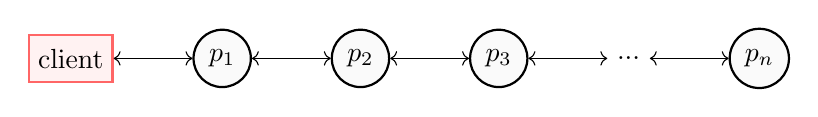
\begin{tikzpicture}[
squarednode/.style={rectangle, draw=red!60, fill=red!5, thick, minimum size=6mm},
roundnode/.style={circle, draw, thick, fill=black!2, minimum size=6mm},
ghostnode/.style={minimum size=5mm},
]
%Nodes
\node[squarednode]      (c0)       {client};
\node[roundnode]        (p1)       [right=of c0] {$p_1$};
\node[roundnode]        (p2)       [right=of p1] {$p_2$};
\node[roundnode]        (p3)       [right=of p2] {$p_3$};
\node[ghostnode]        (px)       [right=of p3] {$...$};
\node[roundnode]        (pn)       [right=of px] {$p_n$};

%Lines
\draw[<->] (c0.east) -- (p1.west);
\draw[<->] (p1.east) -- (p2.west);
\draw[<->] (p2.east) -- (p3.west);
\draw[<->] (p3.east) -- (px.west);
\draw[<->] (px.east) -- (pn.west);
\end{tikzpicture}
\end{center}
Each of the $p_i$ nodes here represents a queue cell which holds a value and are
linked together by bidirectional channels of type $\text{queue}_A$.  As
indicated by the type constructor $\&$, the first queue node $q_1$ first
receives either an $\textsf{ins}$ or $\textsf{del}$ label from the client. In
the case of an $\textsf{ins}$ label, $p_1$ receives a value $v$ of type $A$
(indicated by $\multimap$) from the client.  The $p_1$ node then sends an
$\textsf{ins}$ label to $p_2$ and forwards $v$ to it.  This forwarding process
repeats until the value reaches the end of the queue where a new queue cell
$p_{n+1}$ is allocated to store $v$. On the other hand, if $p_1$ receives a
$\textsf{del}$ label, the type constructor $\oplus$ requires that $p_1$ send
either $\textsf{none}$ or $\textsf{some}$.  The $\textsf{none}$ label is sent to
signify that the queue is empty and ready to terminate (indicated by $\End$).
The $\textsf{some}$ label is sent along with a value of type $A$ (indicated by $\otimes$)
which is the dequeued element. Finally, $p_1$ forwards its channel, connecting to
$p_2$, to the client so that the client may continue interacting with the rest of the queue.

It is clear from the example above that the session type $\textsf{queue}_A$ only lists
what operations a queue should support, but does not specify the expected behavior of
these operations. For instance, it does not specify that an $\textsf{ins}$ operation should
add an element to the back of the queue or that a $\textsf{del}$ operation should return the
element at the front of the queue. A correct implementation needs to maintain all of
these additional invariants not captured by the session type. In fact, due to the under
specification of the $\textsf{queue}_A$ type, it is possible to implement a ``queue''
which simply ignores all $\textsf{ins}$ messages and always returns $\textsf{none}$ on $\textsf{del}$.

% The refinement session types of Das et al.~\cite{das20} partially address this issue by
% using \emph{refinement types} to add more precision to session types. In this approach,
% the queue type is refined to the following:
% \begin{align*}
%   \textsf{queue}[n]_A \triangleq \&\{
%   \textsf{ins}: A \multimap \textsf{queue}[n+1]_A,
%   \textsf{del}: \oplus\{\textsf{none}: !\{n = 0\}. \End, \textsf{some}: !\{1 \leq n\}. A \otimes \textsf{queue}_A\}
%   \}
% \end{align*}
% Here, the type $\textsf{queue}[n]_A$ is parameterized by a natural number $n$ which represents
% the length of the queue. The $\textsf{ins}$ operation is refined to indicate that the length
% of the queue increases by one after an insertion. The $\textsf{del}$ operation is refined
% to indicate that the $\textsf{none}$ label may only be sent when the queue is empty (i.e. $n = 0$)
% and that the $\textsf{some}$ label may only be sent when the queue is non-empty (i.e. $1 \leq n$).
% While refinement session types are able to capture the length changes of the queue,
% ruling out many egregiously wrong implementations, they are still unable to capture the actual
% \emph{functional} behavior of the queue. For instance, a stack-like structure can be implemented
% with the above type as its length changes still comply with the refinements.

To address this issue, we develop \TLLC{}, a dependent session type system which
extends the Two-Level Linear dependent type theory (TLL)~\cite{fu23} with
session-typed concurrency. In \TLLC{}, one could define queues through the following
dependent session type:
\begin{alignat*}{2}
  &\textsf{queue} (\textit{xs} : \textsf{list}\ A) :=\ ?(\ell : \textsf{opr}). \Match\ \ell\ \With \\
  &\qquad\mid \textsf{ins}(v) \Rightarrow \textsf{queue}(\textsf{snoc}(xs, v)) \\
  &\qquad\mid \textsf{del} \Rightarrow
    \Match\ \textit{xs}\ \With
    \ (x :: xs') \Rightarrow\ !(\textsf{sing}\ x). !(\HC{\textsf{queue}(xs')}). \End
    \mid [] \Rightarrow \End
\end{alignat*}
Here, the type $\textsf{queue}(\textit{xs})$ is parameterized by a list $\textit{xs}$
which represents the current contents of the queue. Notice that the type no longer needs
the $\oplus$ and $\&$ type constructors to describe branching behavior. Instead, it uses
type-level pattern matching to inspect the label $\ell$ received from the client.
The \textsf{opr} type which $\ell$ inhabits is defined as a simple inductive type with
two constructors:
\begin{align*}
  \Inductive\ \textsf{opr} := \textsf{ins}: A \rightarrow \textsf{opr} \mid \textsf{del}: \textsf{opr}
\end{align*}
When a queue server receives an $\textsf{ins}(v)$ value, the type of the server becomes
$\textsf{queue}(\textsf{snoc}(xs, v))$ were $\textsf{snoc}$ appends $v$ to the end of $xs$.
Conversely, when a $\textsf{del}$ label is received, the type-level pattern matching on $xs$
enforces that if the queue is non-empty (i.e. $x :: xs'$ case), then the server must send
the front element $x$ of the queue to the client (indicated by the \emph{singleton type}
$\textsf{sing}\ x$) along with the channel $\HC{\textsf{queue}(xs')}$ connecting to the remainder
of the queue. If the queue is empty (i.e. $[]$ case), then the server simply terminates.

Given the \textsf{queue} protocol describe above, we can construct queue process nodes and
interact with them. The following signatures are of helper functions that wrap interactions with
the queue nodes into a convenient interface:
\begin{alignat*}{2}
  &\textsf{insert} &&: \forall \{xs : \textsf{list}\ A\}\;(x: A) \rightarrow \textsf{Queue}(xs) \rightarrow \textsf{Queue}(\textsf{snoc}(xs, x)) \\
  &\textsf{delete} &&: \forall \{x: A\}\;\{xs : \textsf{list}\ A\} \rightarrow
    \textsf{Queue}(x :: xs) \rightarrow \mcC (\textsf{sing}\ x \otimes \textsf{Queue}(xs)) \\
  &\textsf{free}   &&: \textsf{Queue}([]) \rightarrow \mcC(\textsf{unit})
\end{alignat*}
The \textsf{Queue} type here is a type alias for the \emph{channel type} of queues
(explained later in detail) and the $\mcC$ type constructor here is the \emph{concurrency monad}
which encapsulates concurrent computations. Notice in the signature of \textsf{insert} and
\textsf{delete} that there are dependent quantifiers surrounded by curly braces.
These are the \emph{implicit} quantifiers of TLL which indicate that the corresponding arguments
are ``ghost'' values used for type checking and erased prior to runtime. For our purposes here,
such ghost values are especially useful for \emph{relationally} specifying the expected
behaviors of queue interactions in terms of sequential list operations. For instance, the
signature of \textsf{insert} states that the queue obtained after inserting $x$ is related to
the original queue by the list operation $\textsf{snoc}$. Similarly, the signature of
\textsf{delete} states that deleting from a non-empty queue returns the front element $x$.
Even though neither of these $xs$ ghost values exist at runtime, they \emph{statically} ensure
that concurrent processes implementing these interfaces behave like actual queues, i.e.,
are first-in-first-out data structures. In a later section we will show how a generalized
map-reduce algorithm can be implemented and verified using similar techniques.


% It is important to note that these type-level pattern matches are \emph{static} and do not
% incur any runtime overhead. But most crucially, they guarantee that any concurrent program
% implementing this type behaves like an actual queue. Later we will show how a generalized
% map-reduce algorithm can be implemented and verified using similar techniques.

% Another important aspect of \TLLC{} is its ability to specify and reason about ``ghost'' messages
% in protocols using the computational irrelevancy machinery of TLL. Consider the session type encoding
% for an idealized Shannon cipher protocol:
% \begin{align*}
%   H(E, D) &\triangleq \forall \{k : \mcK\}\;\{m : \mcM\} \rightarrow D(k, E(k, m)) =_{\mcM} m
% \qquad\text{(correctness property)}
%   \\
%   \mcE(E, D) &\triangleq
%                !\{k : \mcK\}. !\{m : \mcM\}. !(c : \mcC). !\{p : H(E,D) \times (c =_\mcC E(k, m))\}. \End
% \end{align*}
% Given public encryption function $E: \mcK \times \mcM \rightarrow \mcC$ and
% decryption function $D: \mcK \times \mcC \rightarrow \mcM$, the protocol $\mcE(E,D)$ begins
% by sending \emph{implicit} messages as indicated by the curly braces: key $k$ of type $\mcK$
% and message $m$ of type $\mcM$. These implicit messages are \emph{ghosts} in the sense
% that they are only used for type checking and do not participate in runtime communication.
% During compilation, the sending and receiving of implicit messages are compiled to no-ops.
% Next, an \emph{explicit} ciphertext $c$ of type $\mcC$, indicated by round parenthesis,
% is sent to the client. Explicit messages are actual runtime messages which are sent and received.
% Finally, another implicit message $p$ is sent which is a proof object witnessing the
% correctness property of the protocol: $c$ is obtained by encrypting $m$ with key $k$.
% Observe that for the overall protocol, \emph{only} ciphertext $c$ will be sent at runtime while
% the other messages (secrets) are erased. The Shannon cipher protocol basically forces communicated messages
% to always be encrypted and prevents accidental leakage of plaintext.

Integrating session typed based concurrency into TLL is non-trivial due to the
fact that TLL is a dependently typed functional language. While prior
works~\cite{gay10,wadler12} have successfully combined \emph{classical} session
types with functional languages, its is well known that classical session types
do not easily support recursive session types~\cite{gay20} (needed to express
our \textsf{queue} type).  The main issue is that classical session types are
defined in terms of a \emph{dual} operator which does not easily commute with
recursive type definitions. The addition of arbitrary type-level computations
through dependent types further complicates this matter.  On the other hand,
\emph{intuitionistic} session types~\cite{caires10} eschew the dual operator and
define dual \emph{interpretations} of session types based their \emph{left} or
\emph{right} sequent rules.  Because intuitionistic session types do not rely on
a dual operator, they are able to support recursive session types without
commutativity issues. However, intuitionistic session types are often formulated
in the context of process calculi without a functional layer. To enjoy the
benefits of intuitionistic session types in a functional setting, we develop a
novel form of intuitionistic session types where we separate the notion of
\emph{protocols} from \emph{channel types}. The $\textsf{queue}(\textit{xs})$
type from before is, in actuality, a protocol whereas
$\HC{\textsf{queue}(\textit{xs})}$ is a channel type. In general, a channel type
is formed by applying the $\CH{\cdot}$ and $\HC{\cdot}$ type constructors to
protocols. These constructors provide dual interpretations to protocols,
allowing dual channels of the same protocol to be connected together. For
example, $!A. P$ would be interpreted dually as follows:
\begin{alignat*}{2}
  &\CH{!A. P}\quad &&(\textsf{send message of type } A) \\
  &\HC{!A. P}\quad &&(\textsf{receive message of type } A)
\end{alignat*}
Such channel types can be naturally included into the contexts of functional
type systems without needing to instrument the underlying language into a
sequent calculus formulation.  We believe our treatment of intuitionistic
session types is not specific to \TLLC{} and is widely applicable for
integrating intuitionistic session types with other functional languages.

In order to show that \TLLC{} ensures communication safety, we develop a process
calculus based concurrency semantics. Process configurations in the calculus are
collections of \TLLC{} programs interconnected by channels. At runtime,
individual processes are evaluated using the program semantics of base TLL. When
two processes at opposing ends (i.e. dually typed) of a channel are synchronized
and ready to communicate, the process level semantics transmits their messages
across the channel. We study the meta-theory of \TLLC{} and prove that it is
indeed sound at both the level of terms and at the level of process
configurations.

All lemmas and theorems reported in the this paper are formalized in
Rocq~\cite{coq}. All examples can be compiled into C programs using our prototype
compiler where concurrent processes are implemented using POSIX threads.  The
compiler implements advanced language features such dependent pattern matching
and functional in-place programming~\cite{lorenzen23} for linear types. Proofs,
source code, and examples are available in our git repository\footnote{\TODO}.

In summary, we make the following contributions:
\begin{itemize}
  \item We extend the Two-Level Linear dependent type theory (TLL) with session
        type based concurrency, forming the language of \TLLC{}. \TLLC{} inherits the
        strengths of TLL such as Martin-L\"{o}f style linear dependent types and the
        ability to control program erasure.
  \item We develop a novel formulation of intuitionistic session types
        through a clear separation of protocols and channel types. We believe
        this formulation to be widely applicable for integrating session types into
        other functional languages.
  \item We study the meta-theoretical properties of \TLLC{}. We show that
        \TLLC{}, as a term calculus, possesses desirable properties such as confluence and
        subject reduction and, as a process calculus, guarantees communication safety.
  \item The entire calculus, with its meta-theorems, is formalized in Rocq.
  \item We implement a prototype compiler which compiles \TLLC{} into safe and
        efficient C code.
\end{itemize}


%%% Local Variables:
%%% mode: LaTeX
%%% TeX-master: "main"
%%% End:


\section{Overview of Dependent Session Types}
Session types in \TLLC{} are \emph{minimalistic} in design and yet surprisingly expressive
due to the presence of dependent types. Through examples, we provide an overview of
how dependent session types facilitate verified concurrent programming in \TLLC{}.

\subsection{Message Specification}\label{sec:message-specification}
An obvious, but important, use of dependent session types is the precise specification
of message properties communicated between parties. This is useful in practical network
systems where the content of messages may depend on the value of a prior request.
Consider the following protocol:
\begin{align*}
  !(\textit{sz}: \textsf{nat}).\
  ?(\textit{msg}: \textsf{bytes}).\ ?\{\textsf{sizeOf}(\textit{msg}) = \textit{sz}\}.\ \End
\end{align*}
Informally speaking, this protocol first expects a natural number \textit{sz} to be sent
followed by receiving a byte string \textit{msg}. In simple session type systems without
dependency, there would be no way of specifying the relationship between \textit{sz} and
\textit{msg}. However, dependent session types allow us to express relations between messages.
Notice in the third interaction expected by the protocol, the party sending \textit{msg} must
provide a \emph{proof} that the size of \textit{msg} is indeed \textit{sz} according to
an agreed upon \textsf{sizeOf} function. Finally, the protocol terminates with $\End$ and
communication ends. Notice that the proof here, as indicated by the curly braces, is a
\emph{ghost message}: it is used for type checking and erased prior to runtime. Even though
the proof does not participate in actual communication, the necessity for the send of
\textit{msg} to provide such a proof ensures that the protocol is followed correctly.

This example showcases the main primitives for constructing dependent protocols in
\TLLC{}: the $!(x : A).B$ and $?(x : A).B$ \emph{protocol actions}. The syntax of these
constructs take inspiration from binary session types~\cite{gay10,wadler12} and label
dependent session types~\cite{ldst}, however the meaning of these constructs in \TLLC{} is
subtly different. In prior works, the $!$ marker indicates that the channel is to send
and the $?$ marker indicates that the channel is to receive. In \TLLC{}, neither marker
expresses sending or receiving per se, but rather an abstract action that needs to be
interpreted through a \emph{channel type}. Hence, the description of the messaging protocol
above is stated to be informal. To assign a precise meaning to the protocol, we need to
view it through the lenses of channel types:
\begin{align*}
  &\CH{!(\textit{sz}: \textsf{nat}).\ ?(\textit{msg}: \textsf{bytes}).\ ?\{\textsf{sizeOf}(\textit{msg}) = \textit{sz}\}.\ \End} \\
  &\HC{!(\textit{sz}: \textsf{nat}).\ ?(\textit{msg}: \textsf{bytes}).\ ?\{\textsf{sizeOf}(\textit{msg}) = \textit{sz}\}.\ \End}
\end{align*}
Here, these two channel types are constructed using \emph{dual} channel type
constructors: $\CH{\cdot}$ and $\HC{\cdot}$.  The $\CH{\cdot}$ constructor
interprets $!$ as sending and $?$ as receiving while the $\HC{\cdot}$
constructor interprets $!$ as receiving and $?$ as sending. In other words, dual
channel types interpret protocol actions in opposite ways. These constructors act similarly
to the duality of left and right rules for intuitionistic session types~\cite{caires10}.
Unlike intuitionistic session types which require the base type system to be
based on sequent calculus, our channel types can be integrated into the type
systems of functional languages so long as linear types are supported.

\subsection{Dependent Ghost Secrets}
Dependent ghost messages have interesting applications when it comes to message specification.
Consider the following encoding of a idealized Shannon cipher protocol:
\begin{align*}
  H(E, D) &:= \forall \{k : \mcK\}\;\{m : \mcM\} \rightarrow D(k, E(k, m)) =_{\mcM} m
\qquad\text{(correctness property)}
  \\
  \mcE(E, D) &:=\ !\{k : \mcK\}.\ !\{m : \mcM\}.\ !(c : \mcC).\ !\{H(E,D) \times (c =_\mcC E(k, m))\}.\ \End
\end{align*}
Given public encryption and decryption functions
$E: \mcK \times \mcM \rightarrow \mcC$ and
$D: \mcK \times \mcC \rightarrow \mcM$ respectively, the protocol $\mcE(E,D)$
begins by sending ghost messages: key $k$ of type $\mcK$ and message $m$ of type
$\mcM$.  Next, the ciphertext $c$ of type $\mcC$, indicated by round
parenthesis, is actually sent to the client. Finally, the last ghost message
sent is a proof object witnessing the correctness property of the
protocol: $c$ is obtained by encrypting $m$ with key $k$.  Observe that for the
overall protocol, \emph{only} ciphertext $c$ will be sent at runtime while the
other messages (secrets) are erased. The Shannon cipher protocol basically
forces communicated messages to always be encrypted and prevents the accidental
leakage of plaintext.

It is important to note that ghost messages and proof specifications, by
themselves, are \emph{not} sufficient to guaranteeing semantic security.
An adversary can simply use a different programming language and circumvent the
proof obligations imposed by \TLLC{}. However, these obligations are useful in
ensuring that honest parties correctly follow \emph{trusted} protocols to defend
against attackers. For example, in the Shannon cipher protocol above, an honest
party is required by the type system to send a ciphertext that is indeed encrypted
from the (trusted) algorithm $E$.

Another, more concrete, example of using ghost messages to specify secrets is the
Diffie-Hellman key exchange~\cite{DH76} protocol defined as follows:
\begin{align*}
  \textsf{DH}(p\ g: \textsf{int})
  :=\ & !\{a: \textsf{int}\}.\ !(A: \textsf{int}).\ !\{A = \textsf{powm}(g, a, p)\}.\\
      & ?\{b: \textsf{int}\}.\ ?(B: \textsf{int}).\ ?\{B = \textsf{powm}(g, b, p)\}.\ \End
\end{align*}
The \textsf{DH} protocol is parameterized by publicly known integers $p$ and $g$.
Without loss of generality, we refer to the message sender for the first row of the
protocol as Alice and the message sender for the second row as Bob. From Alice's
perspective, she first sends her secret value $a$ as a dependent ghost message to
initialize her half of the protocol. Next, her public value $A$ is sent as a real
message to Bob along with a proof that $A$ is correctly computed from values $p, g$ and $a$
(using modular exponentiation \textsf{powm}). At this point, Alice has finished sending
messages and waits for message from Bob to complete the key exchange. She first
``receives'' Bob's secret $b$ as a ghost message which initializes Bob's half of the
protocol. Later, Bob' public value $B$ is received as a real message along with a proof
that $B$ is correctly computed from $p, g$ and $b$. Notice that between Alice and Bob,
the only the real messages $A$ and $B$ will be exchanged at runtime. The secret values
$a$ and $b$ and the correctness proofs are all ghost message that are erased prior to
runtime. Basically, the \textsf{DH} protocol forces communication between Alice and Bob
to be encrypted and maintain secrecy at runtime.

\vspace{-0.4em}
\begin{center}
\begin{minipage}{0.45\textwidth}
\begingroup
\small
\addtolength{\jot}{-0.25em}
\begin{alignat*}{4}
  &\Def\ \textsf{Alice}\ (a\ p\ g: \textsf{int})\ (c : \CH{\textsf{DH}(p,g)}) \\
  &: \CM{\textsf{unit}} := \\
  &\quad\Let\ c \Leftarrow \Send\ c\ \{ a \}\ \In \\
  &\quad\Let\ c \Leftarrow \Send\ c\ (\textsf{powm}(g, a, p))\ \In \\
  &\quad\Let\ c \Leftarrow \Send\ c\ \{\textsf{refl}\}\ \In \\
  &\quad\Let\ \langle{\{b\}, c}\rangle \Leftarrow \Recv\ c\ \In \\
  &\quad\Let\ \langle{B, c}\rangle \Leftarrow \Recv\ c\ \In \\
  &\quad\Let\ \langle{\{\textit{pf}\}, c}\rangle \Leftarrow \Recv\ c\ \In \\
  &\quad\Close(c)
\end{alignat*}
\endgroup
\end{minipage}
\begin{minipage}{0.5\textwidth}
\begingroup
\small
\addtolength{\jot}{-0.25em}
\begin{alignat*}{4}
  &\Def\ \textsf{Bob}\ (b\ p\ g: \textsf{int})\ (c : \HC{\textsf{DH}(p,g)}) \\
  &: \CM{\textsf{unit}} := \\
  &\quad\Let\ \langle{\{a\}, c}\rangle \Leftarrow \Recv\ c\ \In \\
  &\quad\Let\ \langle{A, c}\rangle \Leftarrow \Recv\ c\ \In \\
  &\quad\Let\ \langle{\{\textit{pf}\}, c}\rangle \Leftarrow \Recv\ c\ \In \\
  &\quad\Let\ c \Leftarrow \Send\ c\ \{ b \}\ \In \\
  &\quad\Let\ c \Leftarrow \Send\ c\ (\textsf{powm}(g, b, p))\ \In \\
  &\quad\Let\ c \Leftarrow \Send\ c\ \{\textsf{refl}\}\ \In \\
  &\quad\Wait(c)
\end{alignat*}
\endgroup
\end{minipage}
\end{center}
\vspace{0.5em}

The \textsf{DH} key exchange protocol can be implemented through two simple monadic
programs \textsf{Alice} and \textsf{Bob} as shown above. The $\mcC$ type constructor
here is the concurrency monad for integrating the \emph{effect} of concurrent
communication with the \emph{pure} functional core of \TLLC{}. There are two kinds of
\textsf{send} (and respectively \textsf{recv}) operations at play here.
The first kind, indicated by $\textsf{send}\ c\ \{v\}$ is for sending a ghost message
$v$ on channel $c$. After type checking, these ghost sends are compiled to no-ops
to that they do not participate in runtime communication. The second kind, indicated by
$\textsf{send}\ c\ (v)$, is for sending a real message $v$ on channel $c$. These
real sends are compiled to actual messages in the generated code. Finally, the
\textsf{close} and \textsf{wait} operations synchronize the termination of the protocol.
Notice that the duality of channel types $\CH{\textsf{DH}(p,g)}$ and $\HC{\textsf{DH}(p,g)}$
ensure that every send in \textsf{Alice} is matched by a corresponding receive in
\textsf{Bob} and vice versa. Moreover, \textsf{Alice} and \textsf{Bob} are enforced by the
type checker to correctly carry out the Diffie-Hellman key exchange.

%%% Local Variables:
%%% mode: LaTeX
%%% TeX-master: "main"
%%% End:


\section{Relational Verification via Dependent Session Types}
Earlier in the introduction section, we showed a sketch of how dependent session types
can be used for certified concurrent programming through the example of a concurrent queue.
In this section, we provide a detailed account of how we can use dependent session types
to construct a generic map-reduce system. Similarly to the queue example, we will verify
the correctness of the map-reduce system by relating it to sequential operations on trees.

The first step in constructing the map-reduce system is to define the kinds of operations
that can be performed by the system.
\begingroup
\small
\addtolength{\jot}{-0.2em}
\begin{align*}
  \Inductive\ \textsf{opr}(A : \Un) :=\ &\textsf{Free}  : \textsf{opr}(A) \\
  \mid\ &\textsf{Map}   : \forall \{B : \Un\}\ (f : A \rightarrow B) \rightarrow \textsf{opr}(A) \\
  \mid\ &\textsf{Reduce}: \forall \{B : \Un\}\ (f : A \rightarrow B)\ (g : B \rightarrow B \rightarrow B) \rightarrow \textsf{opr}(A)
\end{align*}
\endgroup

%%% Local Variables:
%%% mode: LaTeX
%%% TeX-master: "main"
%%% End:


\section{Formal Theory of Dependent Session Types}
\subsection{Core TLL}
In this section, we give a brief summary of the Two-Level Linear dependent type theory (TLL)~\cite{fu23}. 
TLL is a dependent type theory that combines 
Martin-L\"{o}f-style dependent types~\cite{martinlof} 
with linear types~\cite{girard,wadler1990}. 
Notably, TLL supports \emph{essential linearity}~\cite{luo} through the use of
a stratified ``two-level'' typing system: the \emph{logical} level and the \emph{program} level. 
The typing judgments of the two levels are written as follows:
\begin{center}
\vspace{0.5em}
\begin{tikzpicture}[
    node distance=2.4cm,
    >=stealth, auto,
    every state/.style={rectangle, draw, rounded corners}
]
\node[state, fill=blue!5] (l)                {\small$\Gamma \vdash m : A\ \text{(Logical Typing)}$};
\node[state, fill=red!5]  (p) [right=of l]   {\small$\Gamma ; \Delta \vdash m : A\ \text{(Program Typing)}$};
\path[-latex,transform canvas={yshift=+1.5ex}] (l.east) edge node {\footnotesize{provides types}} (p.west);
\path[-latex,transform canvas={yshift=-1.5ex}] (p.west) edge node {\footnotesize{subjects to verify}} (l.east);
\end{tikzpicture}
\vspace{0.5em}
\end{center}

First, the \emph{logical} level is a standard dependent type system that supports unrestricted 
usage of types and terms. The primary purpose of the logical level is to provide typing rules
for types which will be used at the logical level. For example, the rules for dependent 
function type ($\Pi$-types) formation are defined at the logical level as follows:
\begin{mathpar}
  \inferrule[Explicit-Fun]
  { \Gamma \vdash A : s \\
    \Gamma, x : A \vdash B : r }
  { \Gamma \vdash \PiR{t}{x : A}{B} : t }

  \inferrule[Implicit-Fun]
  { \Gamma \vdash A : s \\
    \Gamma, x : A \vdash B : r }
  { \Gamma \vdash \PiI{t}{x : A}{B} : t }
\end{mathpar}
The symbols $s, r, t$ range over the \emph{sorts} of type universes, i.e. 
$\Un$ or $\Ln$. These sorts are used to classify types into two categories: 
unrestricted types ($A : \Un$) and linear types ($A : \Ln$).
Program level terms which inhabit unrestricted types can be freely duplicated or discarded,
while those which inhabit linear types must be used exactly once.
Note that this usage restriction is \emph{not} enforced at the logical level
as the logical level typing judgment is completely structural.
This is safe because the logical level will never be executed at runtime and 
is only used for type checking and verification. Thus, multiple uses of
a linear resource at the logical level will not lead to any runtime errors.

At the program level, the typing judgment $\Gamma ; \Delta \vdash m : A$ is used to
exclusively type \emph{terms}. In other words, no rules for forming types are defined
at the program level. All the types used in $\Gamma$, $\Delta$, $m$ and $A$ must be well-formed
according to the logical level typing judgment. This typing judgment possesses two contexts:
$\Gamma$ of all variables in scope, and $\Delta$ of all variables that are computationally relevant
in program $m$. Context $\Delta$ is crucial for enforcing linearity at the program level.
For example, consider the $\lambda$-abstraction rules:
\begin{mathpar}
  \inferrule[Explicit-Lam]
  { \Gamma, x : A ; \Delta, x :_s A \vdash m : B \\ 
    \Delta \triangleright t }
  { \Gamma ; \Delta \vdash \lamR{t}{x : A}{m} : \PiR{t}{x : A}{B} }

  \inferrule[Implicit-Lam]
  { \Gamma, x : A ; \Delta \vdash m : B \\
    \Delta \triangleright t }
  { \Gamma ; \Delta \vdash \lamI{t}{x : A}{m} : \PiI{t}{x : A}{B} }
\end{mathpar}
In \textsc{Explicit-Lam}, we can see that the bound variable $x$ is added to
both contexts $\Gamma$ and $\Delta$. This indicates that $x$ is a variable which
can be used both logically (in types and ghost values) through $\Gamma$, and
computationally (in real values) through $\Delta$. On the other hand, in the
\textsc{Implicit-Lam} rule, $x$ is only added to $\Gamma$ but not $\Delta$.
This indicates that $x$ is a ghost variable which can only be used logically.
A ubiquitous example of ghost variables are type parameters in polymorphic functions.
For example, the polymorphic identity function can be implemented as
\begin{align*}
  \lamI{\Un}{A : \Un}{\lamR{\Un}{x : A}{x}}
\end{align*}
which has the type $\PiI{\Un}{A : \Un}{\PiR{\Un}{x : A}{A}}$.
Arguments to implicit functions are typed at the logical level, thus
allowing polymorphic functions to be instantiated with a type as an argument.
Additionally, as demonstrated in the examples of prior sections,
ghost variables also facilitate program verification by statically describing 
abstractions and invariants of program states.

In the two $\lambda$-abstraction rules above, 
the premise $\Delta \triangleright t$ is a simple side condition that states: if
$t = \Un$, then all variables in $\Delta$ must be unrestricted. In other words,
the $\lambda$-abstractions that can be applied unrestrictedly (with $t = \Un$)
are not allowed to capture linearly typed variables from $\Delta$. This is
similar to the restriction imposed on closures implementing the $\textsf{Fn}$
trait (i.e. those that can be called multiple times) in Rust~\cite{rust} where
capturing of mutable references is prohibited. If such a restriction is not
imposed, then evaluating a $\lambda$-abstraction (that captures a linear
variable) twice may lead to unsafe memory accesses such as double frees or
use-after-frees.

The application rules for both explicit and implicit functions are as follows:
\begin{mathpar}
  \inferrule[Explicit-App]
  { \Gamma ; \Delta_1 \vdash m : \PiR{t}{x : A}{B} \\ 
    \Gamma ; \Delta_2 \vdash n : A }
  { \Gamma ; \Delta_1 \dotcup \Delta_2 \vdash \appR{m}{n} : B[n/x] }

  \inferrule[Implicit-App]
  { \Gamma ; \Delta \vdash m : \PiI{t}{x : A}{B} \\ 
    \Gamma \vdash n : A }
  { \Gamma ; \Delta \vdash \appI{m}{n} : B[n/x] }
\end{mathpar}
In \textsc{Explicit-App}, the argument $n$ is a real value which must be typed
at the program level. The $\dotcup$ operator merges the two program context
$\Delta_1$ and $\Delta_2$ by contracting unrestricted variables and requiring
that linear variables be disjoint, thus preventing the sharing of linear
resources. In \textsc{Implicit-App}, the argument $n$ is a ghost value that is
typed at the logical level. Due to the fact that ghost values are erased prior
to runtime, the program context $\Delta$ in the conclusion only tracks the
computationally relevant variables used in $m$. Notice how in \textsc{Explicit-App}, 
the argument $n$ is substituted into the return type $B$. This allows types to depend 
on program level terms regardless of whether they are of linear or unrestricted types.

\paragraph{\textbf{Usage vs Uniqueness}}
Compared to other linear dependent type
theories~\cite{qtt,nothing,llf,vakar14,luo} which only enforce the linear
\emph{usage} of resources, the TLL type system prevents the \emph{sharing} of
linear resources as well. This is similar to the subtle difference between
linear logic~\cite{girard} and bunched implications~\cite{ohearn99,ohearn03}. 
Consider a linear function $f$, in the aforementioned dependent type theories,
of some type $A \multimap B$. When function $f$ is applied to some argument $v$
of type $A$, the argument $v$ is guaranteed to be used exactly once in the 
\emph{body} of $f$. Notice that this notion of linearity does not preclude the
possibility of sharing $v$ with other functions or threads outside of $f$. In
contrast, the shared interpretation of linearity, as described by
O'Hearn~\cite{ohearn03}, require that $v$ be a unique resource which is
exclusively owned by $f$. In other words, $v$ cannot be shared with any other
functions or threads outside of $f$. Wadler, in his seminal
work~\cite{wadler1991}, also made a similar distinction between \emph{linearity}
and \emph{uniqueness} in the context of functional programming, coining the term
\emph{steadfast types} to refer to type systems that enforce both linearity and
uniqueness. In the context of concurrency, the steadfast type system of TLL
makes it especially suitable for integration with session types: linear usage
prevents replaying of communication protocols and uniqueness prevents multiple
threads from simultaneously accessing the same communication channel.

\subsection{Dependent Session Types of \TLLC{}}
In this section, we formally present the dependent session types of \TLLC{}.

\paragraph{\textbf{Protocols and Channel Types}}
As touched on in \Cref{sec:message-specification}, intuitionistic session types
of \TLLC{} are decoupled into \emph{protocols} and \emph{channel types}. 
The rule for forming protocols is as follows:
\begin{mathpar}
  \inferrule[Proto] 
  { \Gamma \vdash }
  { \Gamma \vdash \Proto : \Un }

  \inferrule[Explicit-Action]
  { \Gamma, x : A \vdash B : \Proto }
  { \Gamma \vdash \ActR{\rho}{x : A}{B} : \Proto }

  \inferrule[Implicit-Action]
  { \Gamma, x : A \vdash B : \Proto }
  { \Gamma \vdash \ActI{\rho}{x : A}{B} : \Proto }

  \inferrule[End]
  { \Gamma \vdash }
  { \Gamma \vdash \End : \Proto }

  \text{where } \rho \in \{!, ?\}
\end{mathpar}
Here, the \textsc{Proto} rule introduces the \Proto{} type which is the type of all protocols. 
Note that \Proto{} is an unrestricted type, thus protocols can be freely duplicated or discarded.
The \textsc{Explicit-Action} and \textsc{Implicit-Action} rules form dependent protocols which 
inhabit the \Proto{} type. The \textsc{End} rule marks the termination of a protocol.

\begin{mathpar}
  \inferrule[ChType]
  { \Gamma \vdash A : \Proto }
  { \Gamma \vdash \CH{A} : \Ln }

  \inferrule[Ch]
  { \Gamma ; \Delta \vdash \\ 
    \epsilon \vdash A : \Proto \\ 
    \Delta \triangleright \Un }
  { c :_\Ln \CH{A} ; \Gamma ; \Delta \vdash c : \CH{A} }
\end{mathpar}

\paragraph{\textbf{Concurrency Monad}}

\bibliography{reference}
\end{document}

%%% Local Variables:
%%% mode: latex
%%% TeX-master: t
%%% End:
